\pdfminorversion=4
\documentclass[aspectratio=169]{beamer}

\mode<presentation>
{
\usetheme{default}
\usecolortheme{default}
\usefonttheme{default}
\setbeamertemplate{navigation symbols}{}
\setbeamertemplate{caption}[numbered]
\setbeamertemplate{footline}[frame number] % or "page number"
\setbeamercolor{frametitle}{fg=white}
\setbeamercolor{footline}{fg=black}
\setbeamercolor{footline}{parent=palette primary}
}


\usepackage[utf8x]{inputenc}
\usepackage{courier}
\usepackage{natbib}
\usepackage{array}
\usepackage{tipa}
\usepackage{bold-extra}
\usepackage{minted}
\usepackage[thicklines]{cancel}
\usepackage{fancyvrb}
\usepackage[T1]{fontenc}
\usepackage{lipsum}  
\usepackage{amsmath}
\usepackage{graphicx}
\usepackage{caption}
% \usepackage[russian]{babel}
\usepackage{tikz}
\usetikzlibrary{matrix}
\usetikzlibrary{decorations.pathreplacing} 
\usepackage{hyperref}
\hypersetup{pdfborderstyle={/S/U/W 1}, urlbordercolor=blue}
\usepackage{xcolor}


\xdefinecolor{intensered}{rgb}{1.0,0.0,0.0}
\xdefinecolor{dianablue}{rgb}{0.18,0.24,0.31}
\xdefinecolor{darkblue}{rgb}{0.0,0.28,0.54}
\xdefinecolor{darkgreen}{rgb}{0,0.5,0}
\xdefinecolor{darkgrey}{rgb}{0.35,0.35,0.35}
\xdefinecolor{darkorange}{rgb}{0.8,0.5,0}
\xdefinecolor{darkred}{rgb}{0.7,0,0}
\definecolor{darkgreen}{rgb}{0,0.6,0}
\definecolor{mauve}{rgb}{0.58,0,0.82}
\definecolor{light}{rgb}{0.95,0.95,0.95}
\definecolor{white}{rgb}{255, 255, 255}

\title[DESCRIPTION]{\LARGE Basic Tools for NLP}
%\author{Iuliia Zaitova, Badr M. Abdullah, Prof. Dr. Dietrich Klakow}
\institute{Saarland University}
\author{Rishu Kumar, Iuliia Zaitova, Chris Hyek}

\date{20.04.2023}
\usetikzlibrary{shapes.callouts}
\captionsetup{labelformat=empty,labelsep=none}
\usepackage{etoolbox} 

\newcommand\mybeamerthm[2]{%
  \newtheorem*{#1}{#2}%
  \AtBeginEnvironment{#1}{%
  }%
}

\begin{document}

\logo{\pgfputat{\pgfxy(0.11, 7.4)}{\pgfbox[right,base]{\tikz{\filldraw[fill=white, draw=none] (0 cm, 0 cm) rectangle (20 cm, 1 cm);}\tikz{\filldraw[fill=darkgreen, draw=none] (0 cm, 0 cm) rectangle (2.8 cm, 1 cm);}\mbox{\hspace{-10 cm}
\includegraphics[height=0.9 cm]{Images/saarland-logo.png}}}}} %\includegraphics[height=1 cm]{Images/lsv-logo.png}}}}}

\begin{frame}
  \titlepage
\end{frame}

\logo{\pgfputat{\pgfxy(0.11, 7.4)}{\pgfbox[right,base]{\tikz{\filldraw[fill=white, draw=none] (0 cm, 0 cm) rectangle (80 cm, 1 cm);}\mbox{\hspace{-10 cm}
\includegraphics[height=0.9 cm]{Images/saarland-logo.png}}}}} % \includegraphics[height=1 cm]{Images/lsv-logo.png}}}}}

% Template credit: LSV(UdS), Hackerman Image credit: Pinterest

% START START START START START START START START START START START START START

% \begin{frame}{}
%     \begin{center}
%         \Large WELCOME!
%     \end{center}
% \end{frame}

% \begin{frame}{Indice}
%   \tableofcontents
% \end{frame}

% \section{Logistics}
% \subsection{Motivation}

\begin{frame}{}
\begin{center}
\textbf{Instructors}
\begin{columns}[T]

    \begin{column}{0.3\textwidth}
    \begin{center}
    \textbf{Iuliia Zaitova}
    \begin{figure}
        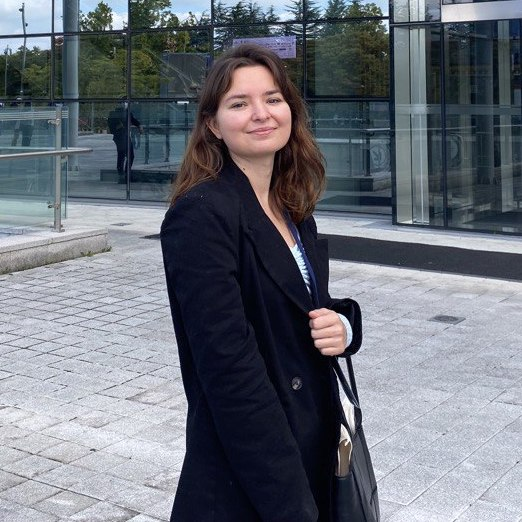
\includegraphics[width=0.8\textwidth, height=0.8\textwidth]{Images/yulia_photo.jpg}
        \caption{ izaitova [at] lsv.uni-saarland.de}
        \label{fig:cockroach}
    \end{figure}
    \end{center}
    \end{column}

    \begin{column}{0.3\textwidth}
    \begin{center}
    \textbf{Rishu Kumar}
    \begin{figure}
        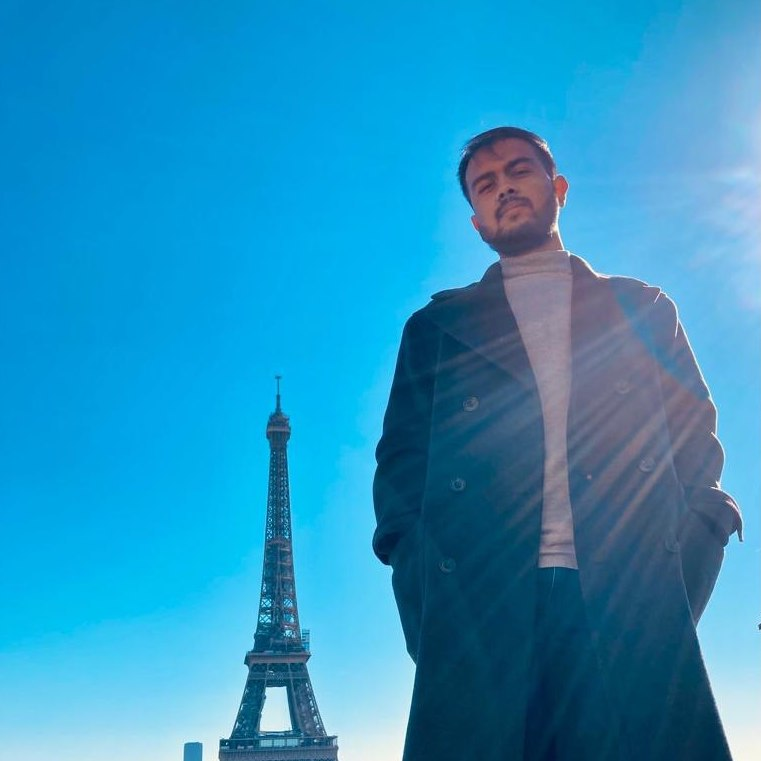
\includegraphics[width=0.8\textwidth, height=0.8\textwidth]{Images/rishu_photo.jpg}
        \caption{riku00002 [at] stud.uni-saarland.de}
        \label{fig:cockroach}
    \end{figure}
    \end{center}
    \end{column}

        \begin{column}{0.3\textwidth}
    \begin{center}
    \textbf{Chris Hyek}
    \begin{figure}
        
\includegraphics[width=0.8\textwidth, height=0.8\textwidth]{Images/chris_photo.jpg}
        \caption{chhy00001 [at] stud.uni-saarland.de}
        \label{fig:cockroach}
    \end{figure}
    \end{center}
    \end{column}
    
\end{columns}
\end{center}
\end{frame}

\begin{frame}{}
    \begin{center}
    \begin{figure}
        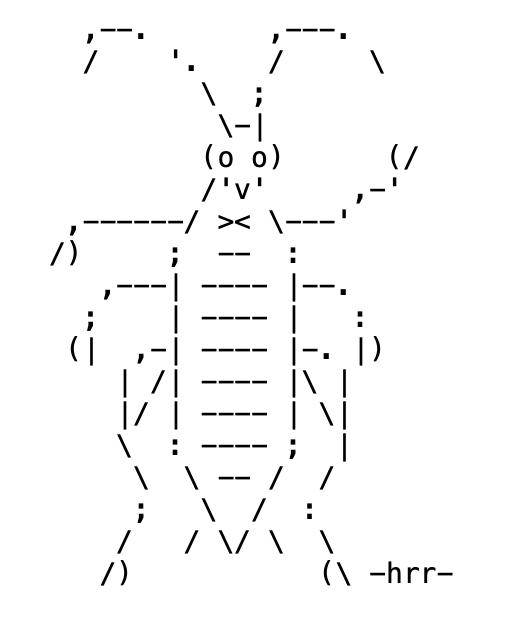
\includegraphics[width=0.6\textwidth, height=0.5\textwidth]{cockroach.png}
        \caption{Obligatory Cockroach Pic}
        \label{fig:cockroach}
    \end{figure}
    \end{center}
\end{frame}


\begin{frame}{Logistics}

\textbf{Logistics:}
\begin{itemize}    
        \item We meet in the same room every Thursday at 16:15
        \item The attendance is optional (of-course)
        \item You are free to attend only the classes which you are interested in
        \item This is a \textit{Dry-Run} for this class, you \textbf{will not} get credits for it
        \item We will try to put (optional) assignments every week
        \item You don't need to submit it anywhere, we can discuss the solution next week
        \item We will use \textbf{Piazza} for discussions
        \item The course material is hosted \href{https://github.com/pyRis/basic-tools-for-NLP}{here}
\end{itemize}

\end{frame}

% \begin{frame}{Links}
% \textbf{Important Links:}
% \begin{itemize}
%     \item bit.ly/btnlp : For Piazza Class
%     \item https://github.com/pyRis/basic-tools-for-NLP : Course Materials
%     \item https://iuliiazaitova.github.io/basic-tools-nlp-2023/ : Course Website
% \end{itemize}
% \end{frame}



\begin{frame}{Important Links:}
\textbf{Important Links:}
\begin{columns}[T]
\begin{column}{0.5\textwidth}
\centering

\includegraphics[width=0.65\textwidth]{Images/qr_code_piazza.jpg} \\
bit.ly/btnlp
\captionof{figure}{Piazza Class}
\end{column}

\begin{column}{0.5\textwidth}
\centering

\includegraphics[width=0.65\textwidth]{Images/qr_code_website.jpg} \\
iuliiazaitova.github.io/basic-tools-nlp-2023
\captionof{figure}{Course Website}
\end{column}
\end{columns}
\end{frame}

\begin{frame}{Links}
\textbf{Objectives:}
\begin{itemize}
    \item Comfortable in tinkering around with your system
\end{itemize}
\end{frame}

\begin{frame}{Links}
\textbf{Objectives:}
\begin{itemize}
    \item Comfortable in tinkering around with your system
    \item Using terminal to make your life easier for tasks
\end{itemize}
\centering

\includegraphics[height=0.4\textwidth,width=0.8\textwidth]{Images/hackerman.png}
\end{frame}

\begin{frame}{Links}
\textbf{Objectives:}
\begin{itemize}
    \item Comfortable in tinkering around with your system
    \item Using terminal to make your life easier for tasks
    \item Introduction to standard tools such as awk, sed, grep
    \item Build your custom pipelines
    \item Refine your coding skills so that it's more ``pythonic'' and Readable
    \item Using version control to keep track of what went wrong
    \item Writing report in \LaTeX/Typst
    \item Using CoLi cluster \textit{the way it's supposed to be used}
\end{itemize}
\end{frame}



\end{document}
